\chapter{Interaction effects on the magneto-optical response of magnetoplasmonic dimers\label{chap4}}

\section{Introduction}

When light is incident over a nanoscale system, its behaviour is strongly dependent of the internal electromagnetic interactions between the constituent elements that form the structure. 
%The possibility of design nanoscale systems almost at will opens the door to the exploitation of unique optical properties in metallic nanostructures. The interaction of light with these small scale systems is strongly dependent of the internal electromagnetic interactions between the constituent elements of the system.  Plasmonic structures composed of a number of individual elements, for example, give rise to Fano resonance effects that lead to electromagnetically induced transparency (EIT) \cite{hentschel2010transition,lassiter2010fano,su2003interparticle, Rechberger_2003,dmitriev2007gold,brown2010heterodimers,wadell2012optical}. 
%In Chap. (\ref{chap3}) a similar phenomenon in magnetoplasmonic nanostructures is presented,  where the system response is externally controlled by a magnetic field \cite{temnov2010active, belotelov2011enhanced,bonanni2011designer,banthi2012high, chin2013nonreciprocal}.\\
With an adequate design of their internal structure, it is possible to obtain configurations which provide enhanced magneto-optical (MO) activity upon plasmon resonance excitation \cite{gonzalez2008plasmonic,jain2009surface,wang2011plasmonics,marinchio2012light}, which allows one to probe the electromagnetic (EM) field distribution inside a metallic nanoelement  \cite{meneses2011probing}, or which yield high MO activity and low optical losses with MO figures of merit comparable with those of garnet structures \cite{banthi2012high}. \\
In the previous chapter, where one of the elements is purely plasmonic and the other is of magnetoplasmonic nature, interaction effects cause the magnetoplasmonic component to induce MO activity in the plasmonic one (which intrinsically lacks MO activity). For specific inter-element distances, which determine the interaction between them, this brings as a consequence the equivalent of the EIT in the MO spectrum of the system, \textit{i.e.}, a cancellation of the MO activity in a narrow spectral range due to the competition between the intrinsic MO contribution of the magnetoplasmonic component and the induced MO contribution of the plasmonic one \cite{armelles2013mimicking}. As this effect exhibits a narrow spectral feature in the MO response, it may find applications in sensing and telecommunication areas, and a complete understanding will help in the development of novel sensing and biosensing architectures as well as MO devices.\\
In this context, these induced MO activity effects and their influence on the overall MO activity of the system for specific ranges of interaction lead to the consideration of additional issues where the electromagnetic interaction between these elements is relevant but remains unaddressed. For example, is it possible to devise a configuration for which the MO activity induced in the non-MO-active element is even larger than that of the MO-active one? Even more, does the MO response depend in a continuous, gradual fashion on the amount of MO-active component? Moreover, in systems where both components are MO active, does the MO response behave simply as the sum of those of the two components?

In this chapter we consider these issues from the theoretical and experimental point of view, by presenting a detailed study of the interaction effects in a model system formed by two coupled nanodisks separated by a dielectric in a nanopillar geometry when the plasmonic or magneto-plasmonic nature of the nanodisk components is changed. Namely, we present results for three different geometries: first, assuming that the bottom disk is magnetoplasmonic and the top one is plasmonic, as in the previous chapter; second, the inverse situation (top magnetoplasmonic, bottom plasmonic); and, finally, the case in which both nanodisks are magnetoplasmonic in nature. For the theoretical description, two approaches are followed: an analytic one in which each disk is considered as a point dipole (with the proper polarisability) and a numerical one based on finite-difference time-domain (FDTD) techniques in which the real internal structure of the disks is taken into account. The first, simple approach allows one to distinguish the contribution of each of the elements separately, giving detailed information about the underlying physics. The second, full numerical approach permits the validation of the obtained insights. These theoretical results are contrasted with the experimental data of equivalent systems obtained by hole mask colloidal lithography and evaporation.


\section{Analytical approach: two interacting dipoles\label{sec:chap4_Discretedipole}}

We consider three different structures each one formed by a two metallic disk elements, vertically aligned, separated by a dielectric spacer, with the top disk smaller than the bottom disk. The disks in each structure can be constituted by gold ($\textnormal{Au}$), or gold and cobalt ($\textnormal{Co}/\textnormal{Au}$), and the dielectric spacer of $\textnormal{SiO}_{2}$. From these materials we obtain the configurations: $\textnormal{Au}/\textnormal{Co}/\textnormal{SiO}_{2}/\textnormal{Au}$, $\textnormal{Au}/\textnormal{SiO}_{2}/\textnormal{Co}/\textnormal{Au}$, and $\textnormal{Au}/\textnormal{Co}/\textnormal{SiO}_{2}/\textnormal{Co}/\textnormal{Au}$.\\ Experimentally the top disk have a thickness of $\approx 16nm$ with a diameter of $\approx 130nm$, the bottom disk have a thickness of $\approx 22nm$ with a diameter of $\approx 150nm$ and the dielectric spacer a thickness of $\approx 20nm$. A detailed description of the fabricated disks can be found in Refs. \cite{dmitriev2007gold, banthi2012high}.\\
Due to the small size of the disks when compared with the wavelength, we can approximate each disk by a single dipole with oblate spheroid shape and an aspect ratio that corresponds to the dimensions of the real disks. In Fig.  (\ref{fig:chap5_schemetic_representation}) we present a schematic representation of these systems.

\begin{figure}[h!]
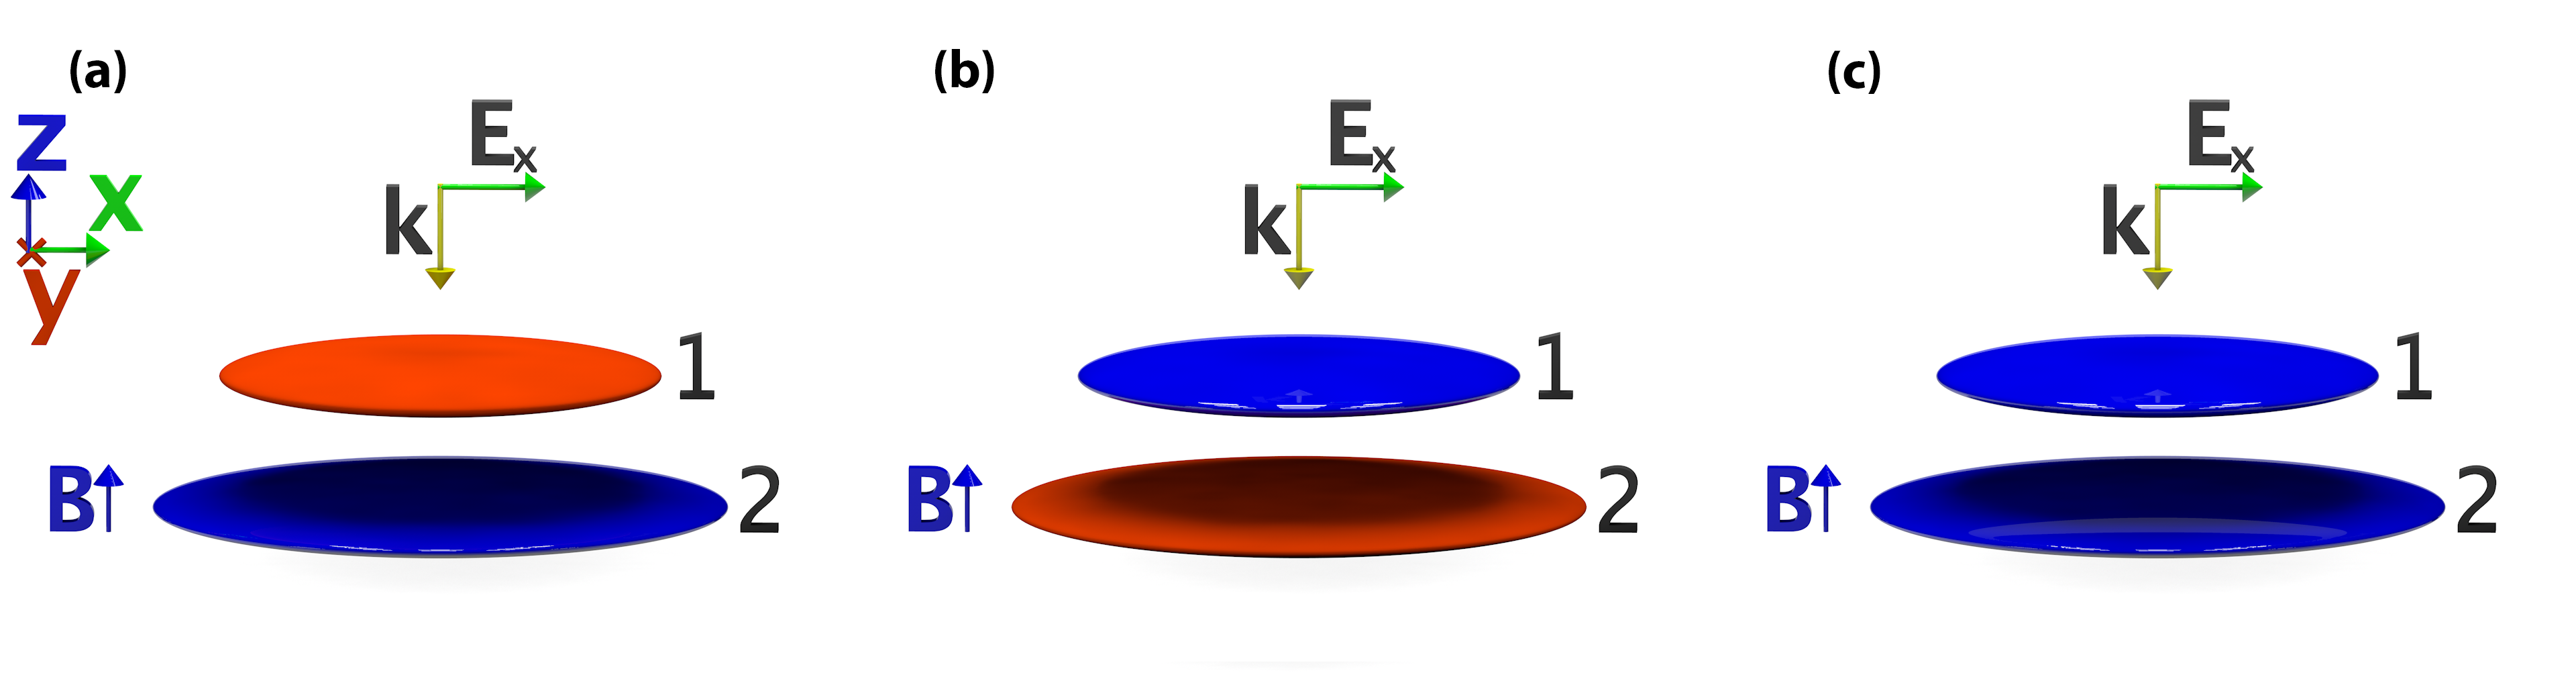
\includegraphics[width=1\columnwidth]{chapter_4/schemes/F1_join_aR1.png}
\caption{ Schematic representation of the studied configurations.\protect \\
 (a) The lower dipole is MP whereas the upper one is P, (b) the lower dipole is P whereas the upper disk is MP, (c) both disks are MP.\label{fig:chap5_schemetic_representation}}
\end{figure}


Since the actual fabricated structures have a truncated cone shape, the aspect ratio of the bottom dipole must be larger than that of the top one. For non-magneto-optical, plasmonic dipoles (P), we consider a diagonal, isotropic, dispersive dielectric tensor ($\textnormal{Au}$). For the magnetoplasmonic (MP) dipole, we consider an average medium that combines the dielectric tensor of a noble metal and that of a ferromagnetic one ($\textnormal{Au}$ and $\textnormal{Co}$ in this case), giving rise to a nondiagonal dielectric tensor. The nonzero off-diagonal elements depend on the relative orientation of the geometry, of the exciting radiation, and of the magnetic field as in the previous case. In our case, the external magnetic field is aligned perpendicular to the dipoles (\textit{i.e.}, aligned along the stacking direction; as schematically presented in Fig. (\ref{fig:chap5_schemetic_representation})), which corresponds to the so-called polar Kerr configuration, and the dielectric tensor of the MP dipole presents the form:

\noindent 
\begin{equation}
\boldsymbol{\epsilon}=\begin{pmatrix}\epsilon_{\text{d}} & \epsilon_{\text{M}} & 0\\
-\epsilon_{\text{M}} & \epsilon_{\text{d}} & 0\\
0 & 0 & \epsilon_{\text{d}}
\end{pmatrix}.\label{Tensor}
\end{equation}


Depending of the amount of $\textnormal{Co}$ within the MP disk, the elements of the dielectric tensor read as: 

\noindent 
\begin{equation}
\boldsymbol{\epsilon}_{\text{{d}}}=\left(1-\nu\right)\boldsymbol{\epsilon}_{\text{d,Au}}+\nu\boldsymbol{\epsilon}_{\text{d,Co}};\:\:\:\boldsymbol{\epsilon}_{\text{{M}}}=\nu\boldsymbol{\epsilon}_{\text{M,Co}}\label{Concent},
\end{equation}
 

where $\nu=\frac{V_{Co}}{V_{Co}+V{}_{Au}}$ is the $\textnormal{Co}$ relative amount in each dipole.

Once the dielectric tensor is known, we evaluate the static polarisability taking into account the properties of the particles, such as the shape (that in this case is oblate), material properties and dimensions. In order to conserve the energy, to the static polarisability is applied the radiative correction. The procedure used here is equivalent to the one presented in the previous chapter, in particular, we use Eq. (\ref{eq:chap3_polarizability}) and Eq. (\ref{eq:chap3_radiative_correction}) for polarisability and radiative correction respectively. \\

Knowing the polarisability for oblate particles, we are able to describe each disk as a single dipole. From coupled dipole theory, we know that the interaction between dipoles is mediated by the Green tensor $\mathbf{G}$. If an incident planar wave, with wave number $k$ and with electric polarisation in the plane of the dipoles, is used to excite the system (see Fig. (\ref{fig:chap5_schemetic_representation})) the two dipoles can be described in the $x-y$ plane as: 

\begin{eqnarray}
\mathbf{p}_{1} & = & \epsilon_{0} \boldsymbol{\alpha}_{1}\left[\mathbf{E}_{0,1}+\frac{k^2}{\epsilon_{0}}{G}\left(\mathbf{r}_{1},\mathbf{r}_{2}\right)\mathbf{p}_{2}\right]\nonumber \\
\mathbf{p}_{2} & = & \epsilon_{0} \boldsymbol{\alpha_{2}}\left[\mathbf{E}_{0,2}+\frac{k^2}{\epsilon_{0}}{G}\left(\mathbf{r}_{2},\mathbf{r}_{1}\right)\mathbf{p}_{1}\right],\label{Twodip}
\end{eqnarray}
which is the same equation obtained in the previous chapter. Due to the symmetry of the problem, the Green tensor is already defined in Eq. (\ref{eq:chap3_greenf}),  being $d$ the distance between dipoles, and $G\left(\mathbf{r}_{1},\mathbf{r}_{2}\right)$.\\


%\begin{eqnarray}
%G({\bf r}_{1},{\bf r}_{2}) & = & {G}({\bf r}_{2},{\bf r}_{1})=\mathcal{G}\mathbb{I}_{2\times2}=\frac{e^{ikr}}{4 \pi r}\left(\frac{(kr)^{2}+ikr-1}{(kr)^{2}}\right)\mathbb{I}_{2\times2},\nonumber \\
%\boldsymbol{\alpha}_{i} & = & \left(\begin{array}{cc}
%\alpha_{i} & \alpha_{iM}\\
%-\alpha_{iM} & \alpha_{i}
%\end{array}\right)
%\end{eqnarray}
The general solution of that system of equations under the influence of a plane wave linearly polarised along the $x-$axis and amplitude $E_{0}$ at dipole $1$ is given by:

\begin{eqnarray}
p_{1x}&=&\epsilon_{0}\frac{E_0}{\mathcal{D}}\left[\alpha_1+k^2 \mathcal{G}e^{-ikd}(\alpha_2\alpha_1-\alpha_{2M}\alpha_{1M})-k^4 \mathcal{G}^2\alpha_2D_1-k^6 \mathcal{G}^3e^{-ikd}D_1D_2\right]\nonumber\\
p_{2x}&=&\epsilon_{0}\frac{E_0}{\mathcal{D}}\left[e^{-ikd}\alpha_2+k^2\mathcal{G}(\alpha_2\alpha_1-\alpha_{2M}\alpha_{1M})-k^4\mathcal{G}^2e^{-ikd}\alpha_1D_2-k^6\mathcal{G}^3D_1D_2\right]\nonumber\\
p_{1y}&=&\epsilon_{0}\frac{E_0}{\mathcal{D}}\left[-\alpha_{1M}-k^2\mathcal{G}e^{-ikd}(\alpha_1\alpha_{2M}+\alpha_2\alpha_{1M})-k^4\mathcal{G}^2\alpha_{2M}D_1\right]\nonumber\\
p_{2y}&=&\epsilon_{0}\frac{E_0}{\mathcal{D}}\left[-e^{-ikd}\alpha_{2M}-k^2\mathcal{G}(\alpha_1\alpha_{2M}+\alpha_2\alpha_{1M})-k^4\mathcal{G}^2e^{-ikd}\alpha_{1M}D_2\right],
\label{eq:chap5_dipoles}\end{eqnarray}where $\mathcal{D}=1-2k^4\mathcal{G}^2(\alpha_2\alpha_1-\alpha_{2M}\alpha_{1M})+k^8\mathcal{G}^4D_1D_2$,
and $D_i=\alpha_i^2+\alpha_{iM}^2$. This equation is in fact a generalisation of Eq. (\ref{eq:chap3_polarizations_solution}). Note that the $y-$component of both dipoles is not zero when at least one of the dipoles is MO active.\\
For the particular geometry we are analysing, the external magnetic field produces a change in the polarisation state of the
reflected light, and the magneto-optical activity (MOA) of the whole system, defined as the modulus of the complex Kerr rotation, can be written as:

\begin{eqnarray}
\text{MOA}&=&|\theta+i\phi|=\textnormal{atan}\frac{\left|E_{y}^{R}\right|}{\left|E_{x}^{R}\right|}\approx\left|\frac{p_{1,y}+p_{2,y}}{p_{1,x}+p_{2,x}}\right|\nonumber \\ 
& = & \frac{(|p_{1,y}|^{2}+|p_{2,y}|^{2}+2|p_{1,y}||p_{2,y}|\cos(\Delta))^{\frac{1}{2}}}{(|p_{1,x}|^{2}+|p_{2,x}|^{2}+2|p_{1,x}||p_{2,x}|\cos(\Gamma))^{\frac{1}{2}}}.\label{CRot}
\end{eqnarray}

From the interaction point of view, there are three different regimes that are determined by the distance between the interacting dipoles: strong interaction (very close dipoles), weak interaction (very far away objects), and medium interaction (intermediate distance). We will concentrate on the most interesting case of medium interactions \cite{armelles2013mimicking}, and will analyse two situations: one in which the amount of $\textnormal{Co}$ in the magneto-optical disk is very small ($0.1\%$) and a second one where it is comparable to the $\textnormal{Au}$ amount ($25\%$). For the analysis, the aspect ratios of the dipoles are $a/c = 13$ and $10$ for the bottom and top dipoles, respectively.\\
\begin{figure}[h!]
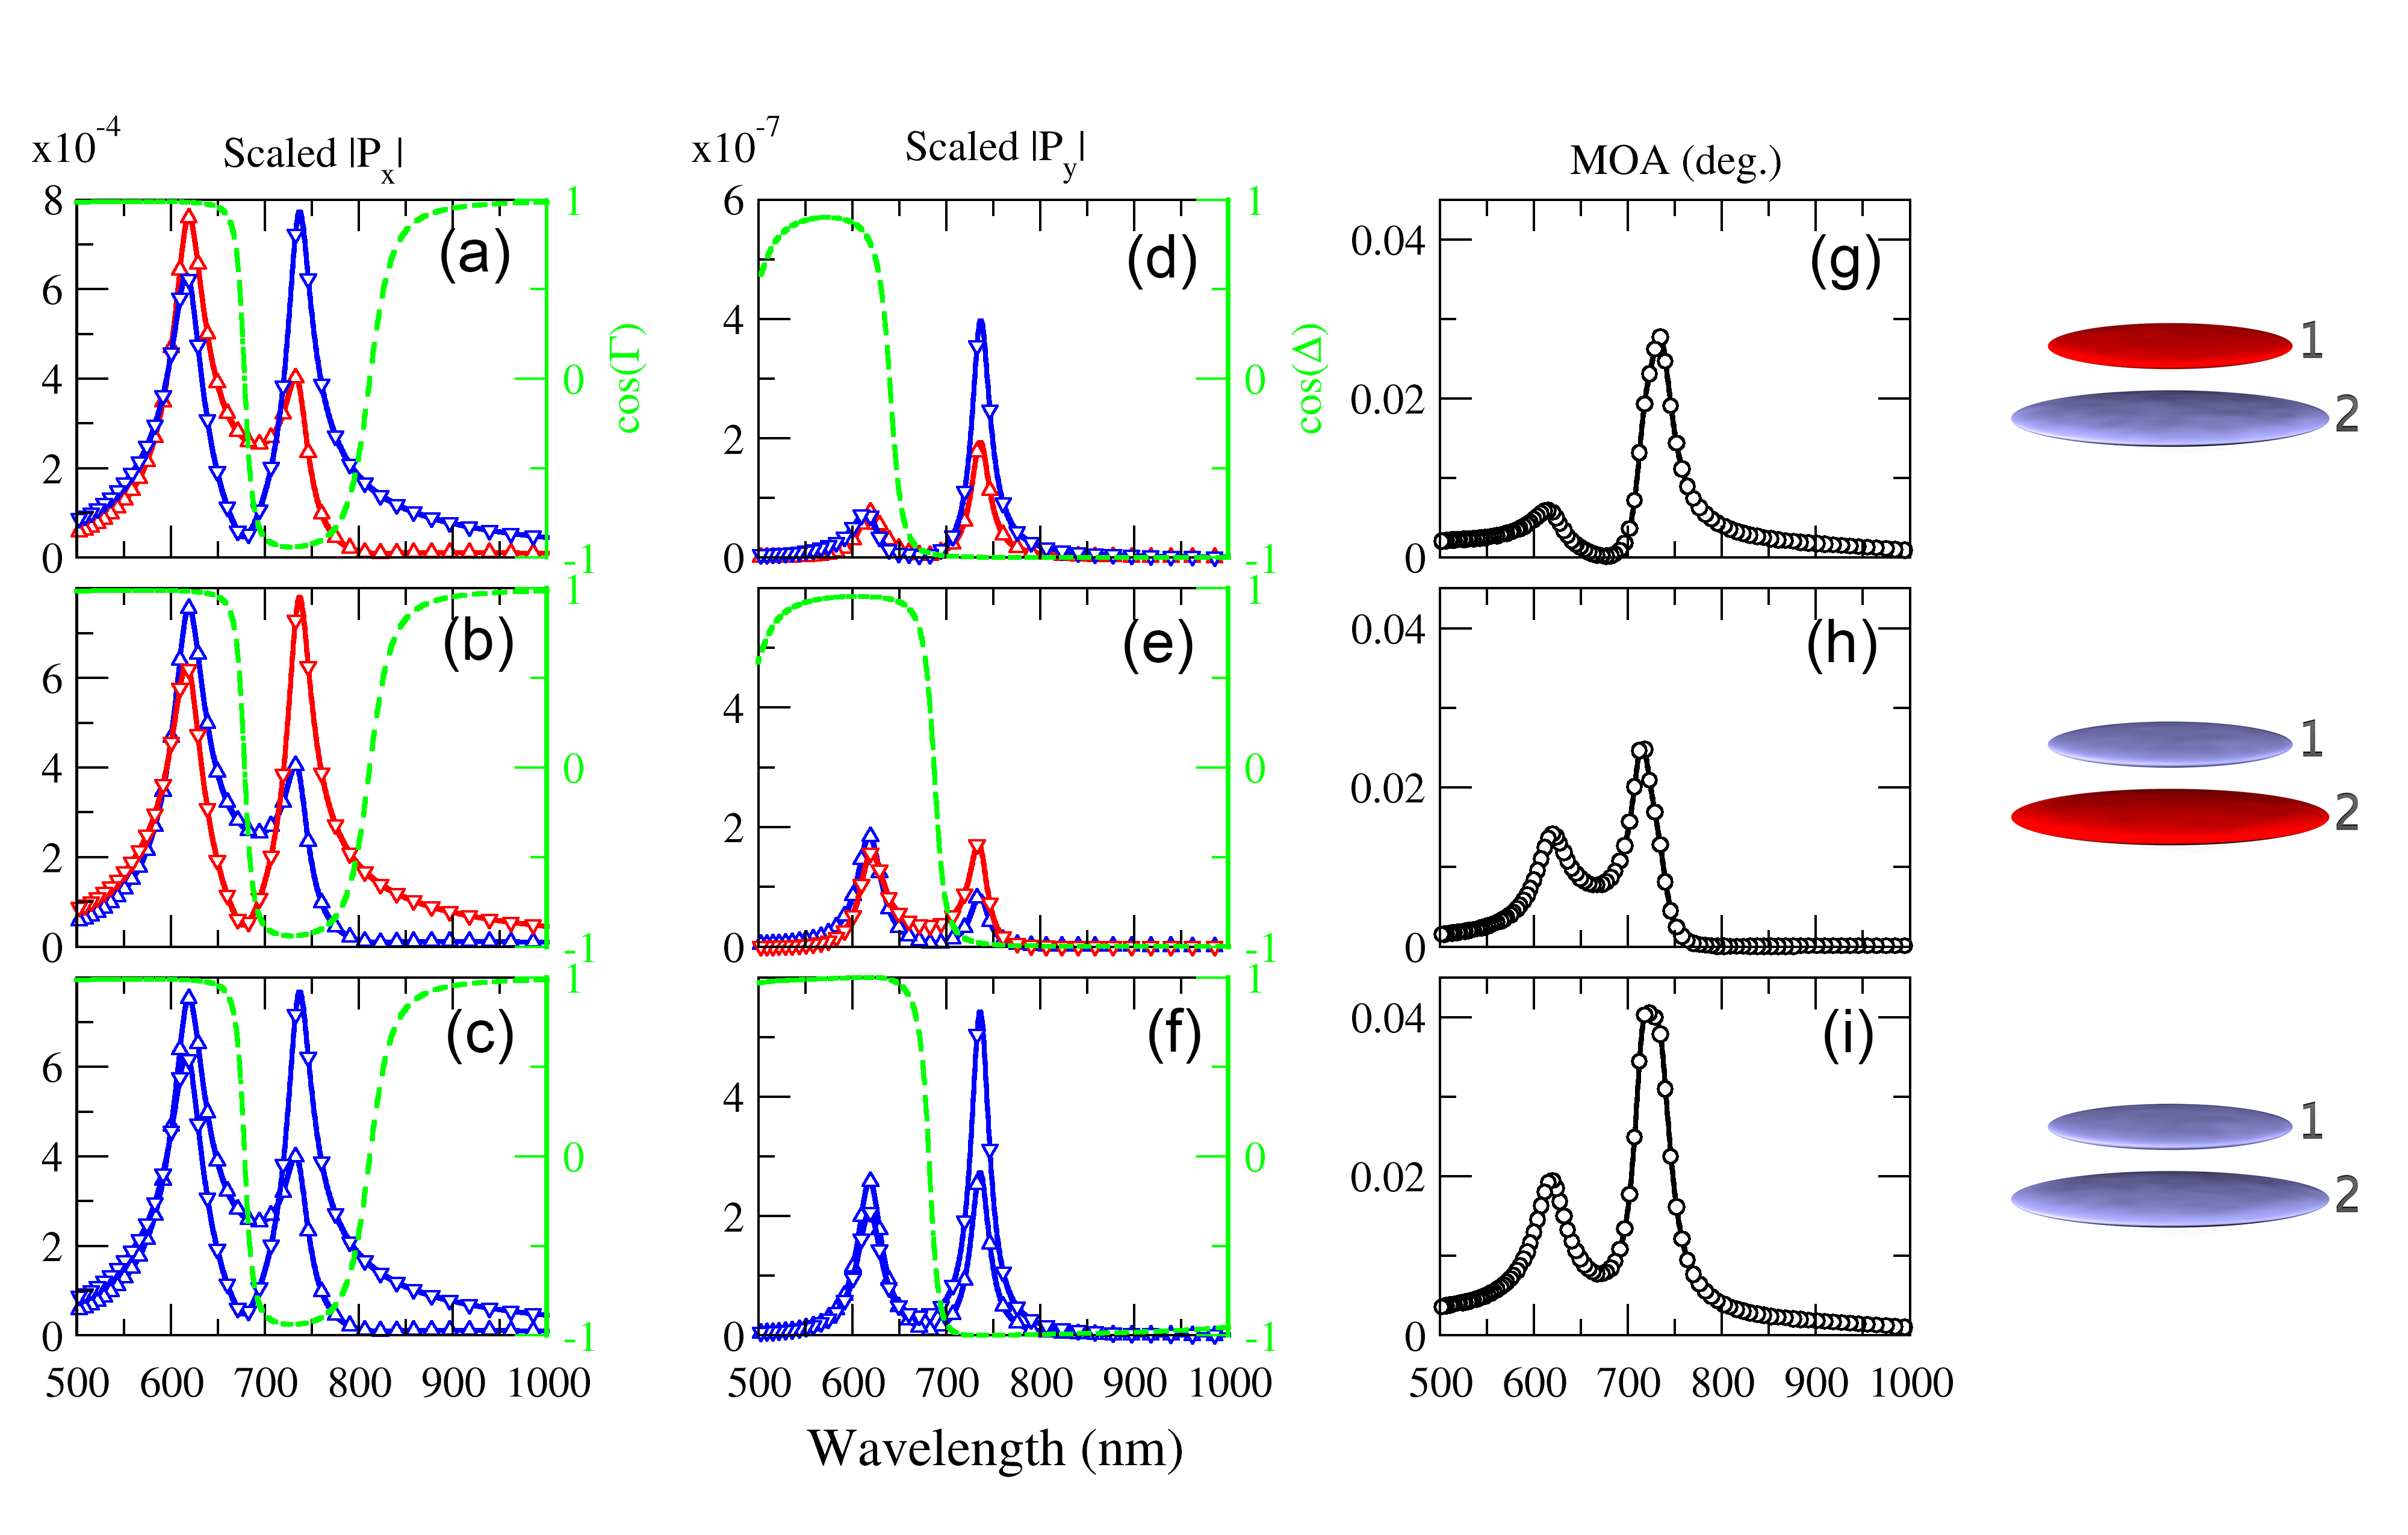
\includegraphics[width=1.0\textwidth]{chapter_4/graphics/F2_lowMO.png}
\caption{Dipole contributions, and MOA for 0.1\% Co concentration. (a)-(c) $x-$component of the scaled dipole (left axis) and the cosine of the relative phase between them (right axis), (d)-(f) $y-$component of the scaled dipole (left axis), and their relative phase (right axis), (g)-(i) magneto-optical activity. The upper panels represent the situation where the MP dipole is at the bottom, the medium panels are when the MP dipole is at the top, the lower panels when both are MP. Triangle-up for the top dipole, and triangle down for the bottom dipole.\label{LowInt}}
\end{figure}
Let us start with the case of very small $\textnormal{Co}$ concentration ($0.1\%$) in the MP dipole. In Fig. (\ref{LowInt}), we show the modulus of the components of the dipole along $x$, the polarisation direction of the incident beam ($p_{i,x}$), and along the $y-$direction ($p_{i,y}$), as well as that of the complex Kerr rotation (MO activity, MOA) calculated with this simple analytical model for the situations where the MP dipole is at the bottom, top, and in both positions of the structure. The cosine of relative phases between the $p_{i,x}$, $\cos\Gamma$ presented in Figs. \ref{LowInt}(a)-\ref{LowInt}(c), and $p_{i,y}$, $\cos\Delta$ presented in Figs. (\ref{LowInt})(d)-(\ref{LowInt})(f), components of the upper and lower disks (dashed curves) are also shown, with limit values of $1$ and $-1$ for in-phase and out-of-phase oscillations, respectively.\\
Considering first the $x-$component of the dipoles, shown in Figs. (\ref{LowInt})(a)-(\ref{LowInt})(c), and due to the low $\textnormal{Co}$ concentration, there is no noticeable difference between the three situations. All cases show two characteristic low-energy ($740nm$) and high-energy ($620nm$) modes of antisymmetric and symmetric nature, respectively \cite{dmitriev2007gold,armelles2013mimicking,banthi2012high}, as directly concluded by the obtained relative phase between the two dipoles. The abrupt change in sign of the cosine occurs exactly at the minimum in magnitude of both dipoles. For energies below roughly $760nm$, the phase gradually changes again, going back to an in-phase configuration for wavelengths larger than $820nm$. Regarding the relative contribution of both disks to these $p_{x}$ spectral features, the low-energy mode has a stronger component originating from the bottom disk (down triangles) than from the top one (up triangles), since it has a lower aspect ratio. The situation is reversed for the high-energy peak, even though the difference between the contributions of the two dipoles is smaller.\\
Beyond the purely optical properties, fully understandable by simply considering $p_{x}$, the direct consequence of the application of a magnetic field is the generation of a $y-$component in the dipole \cite{sepulveda2010plasmon,armelles2013mimicking} (Fig. (\ref{LowInt})(d)-(f)). Contrary to what is observed in the $x-$component, now different results are obtained depending on the specific position of the MP-active dipole.\\
Let us examine each situation individually. When the MP dipole is at the bottom, a $y-$component is observed not only in this dipole, but also in the P top one, which is due to the interaction between the dipoles. This $y-$component is stronger for the bottom MP dipole in the low-energy region, but they are similar in the high-energy region. Even more, in the spectral region, where the $x-$component of the MP dipole is minimum, the $y-$component of both dipoles is almost zero, even though the $x-$component of the P dipole in the same intermediate region is not negligible. This is simply due to the fact that the $y-$component is originated by the magnetic-field-induced rotation of the MP dipole, which in turn induces the rotation of the upper P dipole. Thus, a $y-$component dipole can be originated only if the $x-$component of the MP active dipole is not zero. Additionally, the relative phases between the two dipoles along the $y$ axes show essentially the same symmetric/antisymmetric configuration for the corresponding high/low-energy modes compared to those for the $x-$components, even though now they do not return to in-phase values for energies below $800nm$. The presence of $p_y$ is directly related to the presence of MO activity in the system (see Fig. (\ref{LowInt})(g)). Indeed, as shown in Eq. (\ref{CRot}), this magnitude is basically the modulus of the sum of the $y-$components of the top and bottom dipoles divided by that of the $x-$components. Therefore, the spectral dependence of MOA can be understood in simple terms considering these four dipole components, taking into account their relative phases. So, in this first considered case with the bottom MP dipole, the high-energy peak results from the addition of both (top and bottom dipoles) $y-$components, while the low-energy one results from the corresponding difference, since in this energetic range the $y-$components are in phase opposition.\\
If we consider now the situation where the MP dipole is on the top of the structure, the results are very different. Strikingly, here the obtained $y-$component in the low-energy region is larger for the P dipole than for the MP one, while both components are similar for the high-energy region. This means that the contribution to the MOA coming from the P dipole in the low-energy region is actually stronger than that of the MP one, as shown in Fig. (\ref{LowInt})(h). This is simply due to the larger $x-$component of the P dipole in the low-energy region, which also explains why the $y-$components in the high-energy region are of similar magnitude for both the MP and P dipole in the previous case. On the other hand, regarding the intermediate spectral region, and due to the nonvanishing $x-$component of the MP dipole in this range, both the $y-$components (especially of the P dipole) and the MOA are not zero.
Finally, if both disks have an MO component, the intensity of the $p_y$ components increases for both dipoles, and, within each mode, they follow the same trend as the corresponding $x-$component. Besides, for all of the energy regions, the  intensity of the MOA is larger than that of the other two configurations. 

\begin{figure}
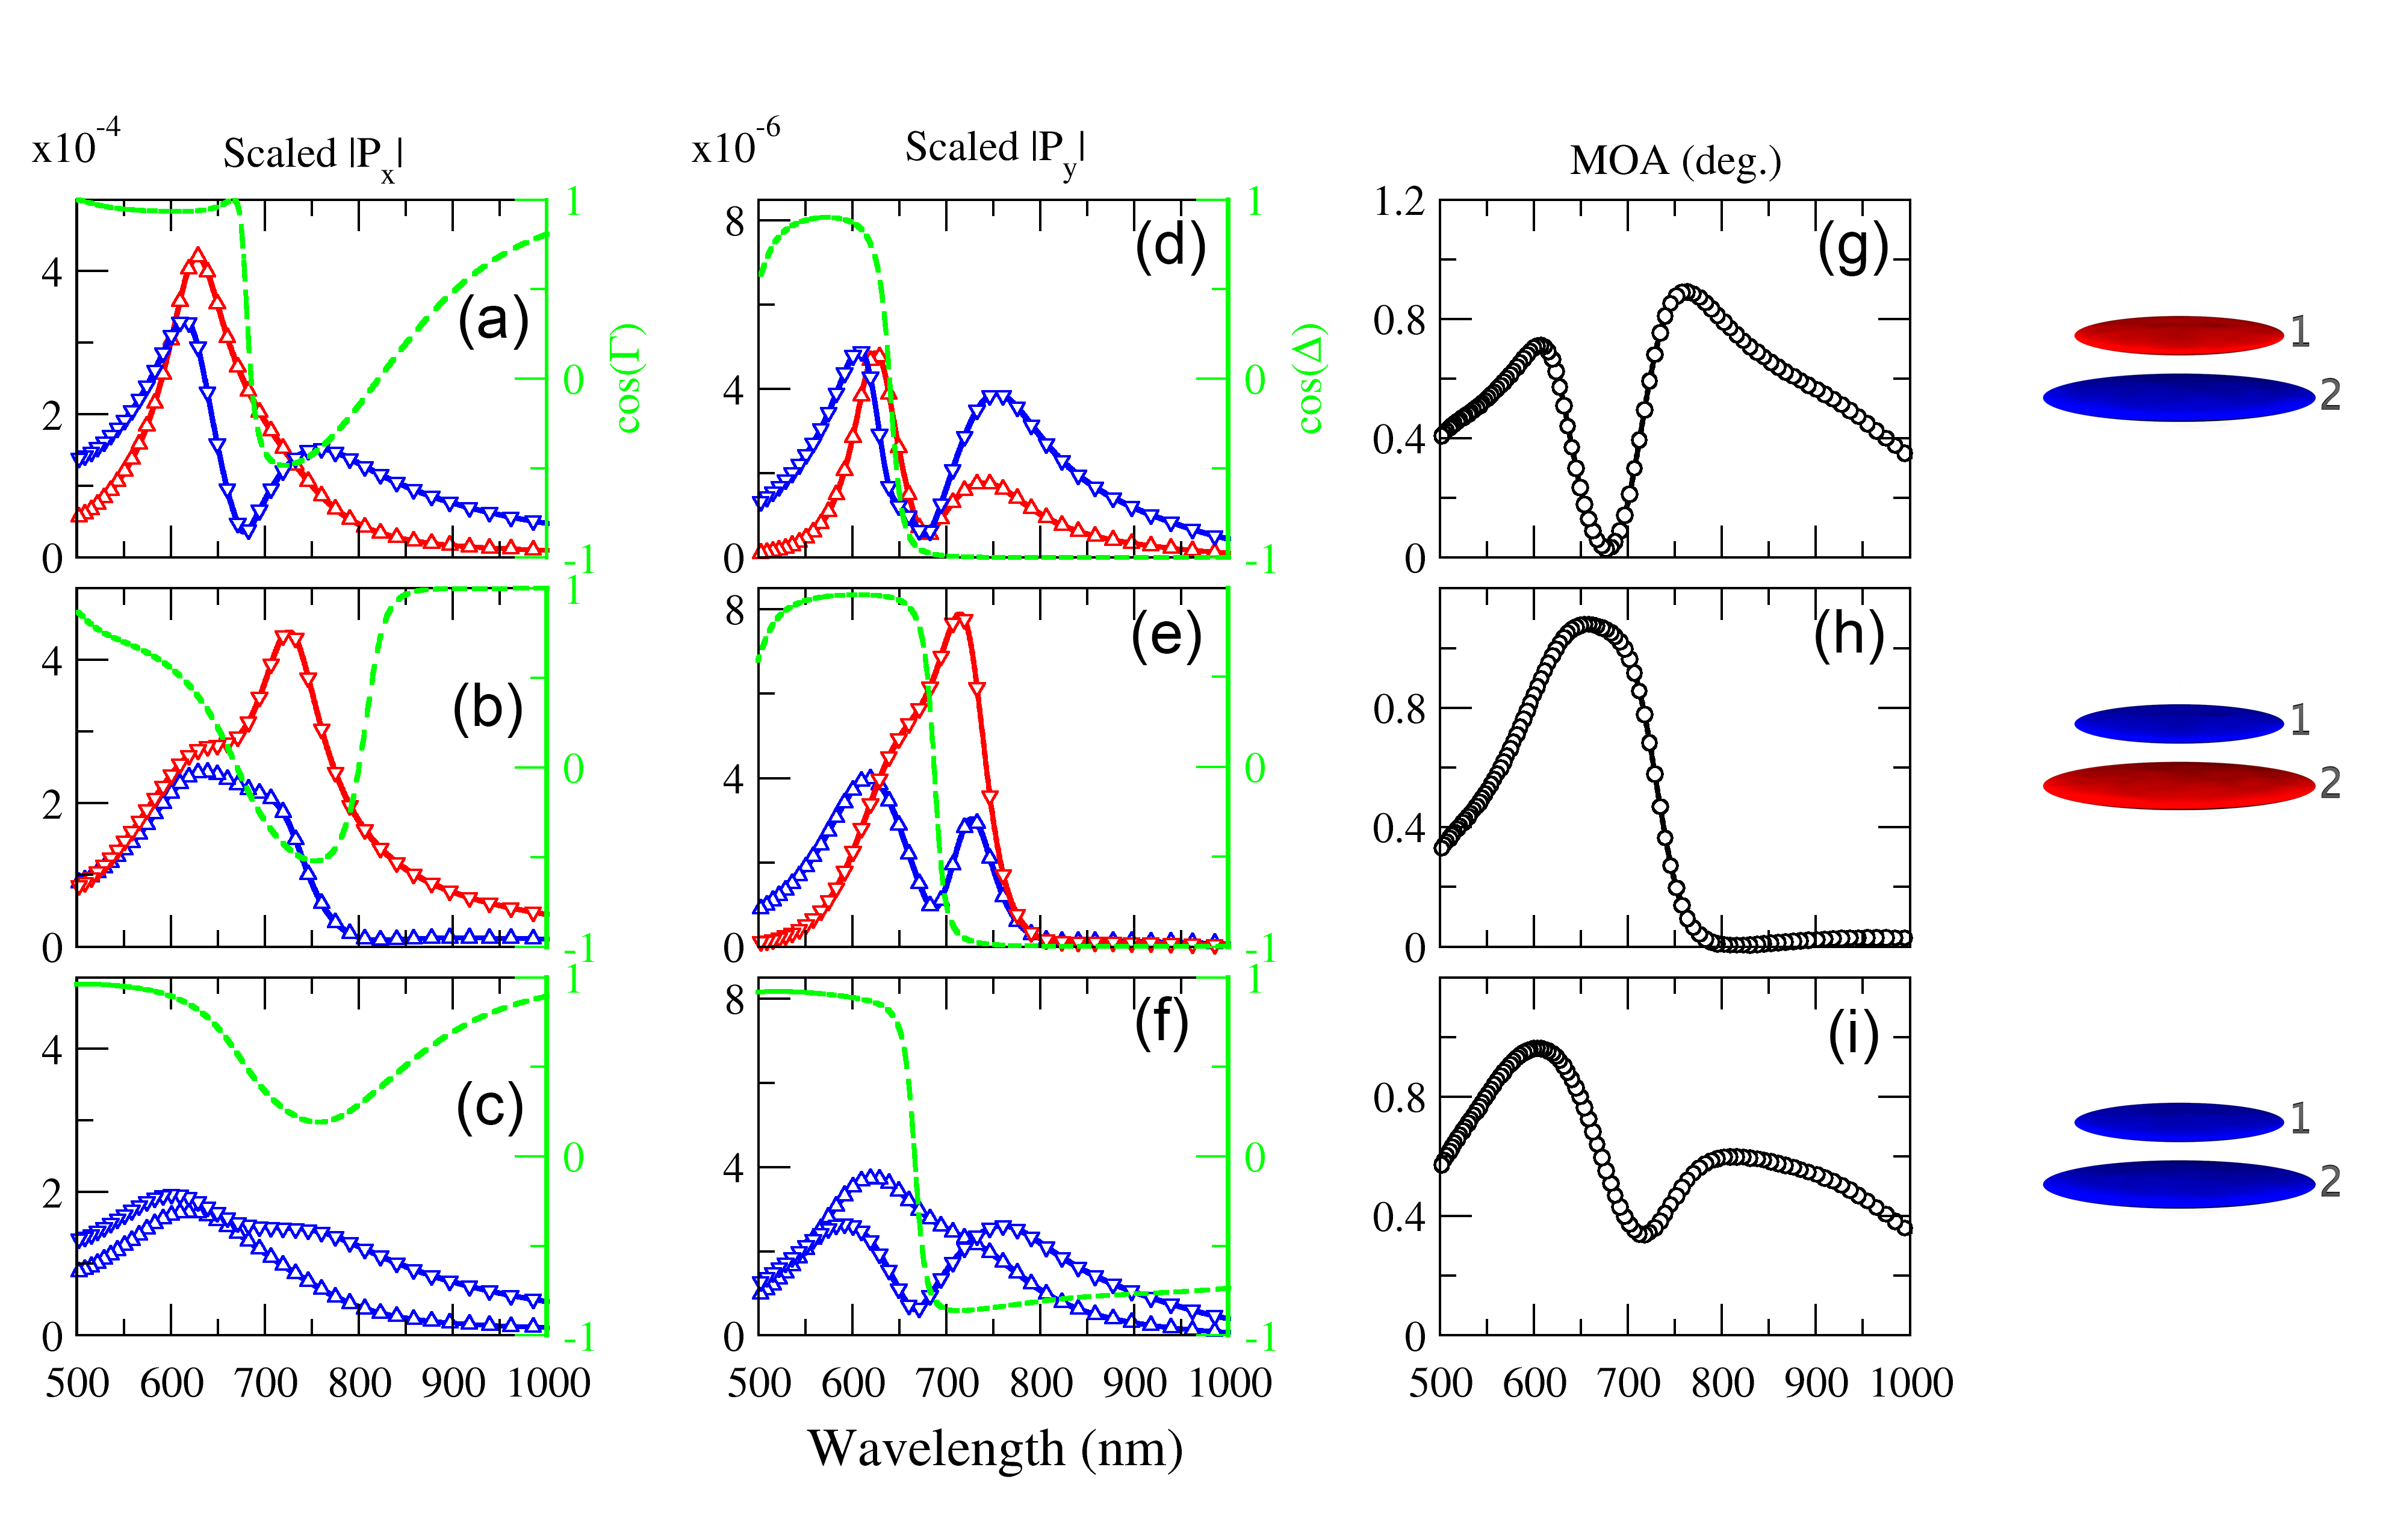
\includegraphics[width=1\textwidth]{chapter_4/graphics/F3_highMO.png}

\caption{Dipole contributions, and MOA for 25\% $\textnormal{Co}$ concentration. (a)-(c) $x-$component of the scaled dipole (left axis) and the cosine of the relative phase between them (right axis), (d)-(f) $y-$component of the scaled dipole (left axis), and their relative phase (right axis), (g)-(i) magneto-optical activity. The upper panels represent the situation where the MP dipole is at the bottom, the medium panels are when the MP dipole is at the top, the lower panels when both are MP. Triangle-up for the top dipole, and triangle down for the bottom dipole \label{HighInt}}
\end{figure}

Going towards a more realistic situation, with larger $\textnormal{Co}$ amounts in the MP dipoles, in Fig. (\ref{HighInt}) we show theoretical calculations equivalent to those shown in Fig. (\ref{LowInt}) but using the dipole model with a $25\%$ $\textnormal{Co}$ content in the different MP dipoles. As can be seen in Figs. (\ref{HighInt})(a)-(\ref{HighInt})(c), and contrary to what was observed for low $\textnormal{Co}$ concentrations, now the $p_x$ components are very different depending on the specific position MP dipole. The effect of increasing the $\textnormal{Co}$ amount is both to broaden the peaks and to change their absolute and relative intensities, as well as their energetic position, both for $p_x$ and $p_y$ components. Due to the much larger amount of $\textnormal{Co}$ ($250$ times more $\textnormal{Co}$) in this case, the magnitudes of the $p_x$ and $p_y$ components are now very different (between a factor of $2$ to $4$ reduction in the $x-$component due to the increased losses, and roughly one order of magnitude larger in the $y-$component due to the much larger amount of MO material). Even more, for this concentration, all of these effects also depend on the specific location of the MP dipole.\\
For the configuration with the MP dipole at the bottom, the low-energy peak in the MOA has a stronger component due to the bottom dipole (as seen in the low $\textnormal{Co}$ concentration case) and the increase of the $\textnormal{Co}$ amount brings, as a consequence, both a reduction of the relative intensity for the $x-$component and a broadening for both the $x-$ and $y-$components. However, the high-energy peak, with a stronger contribution from the upper P dipole, is less affected since no $\textnormal{Co}$ is present in it. Again, a minimum in the $y-$component in the intermediate-energy region yields a minimum in the MO activity. Regarding the relative phases, for the $p_x$ components, it is clear now that they do not reach the perfect out-of phase configuration, indicating that now the nature of the modes is not purely but only partially antisymmetric. This is due to the sizable amount of $\textnormal{Co}$ present in the dipoles, which enhances the losses of the system and affects the retardation between the two coupled dipole $x-$components. However, for the $y-$components, the phase basically reproduces the same behaviour observed for the very low concentration limit.\\
Going now to the situation where the MP dipole is in the upper part, the most affected peak (for all $p_x$, $p_y$, and MOA) due to the incorporation of $\textnormal{Co}$ is the high-energy one, since it is the one which carries a stronger part of the upper dipole. We therefore observe a change in the relative intensity with respect to the case with the MP dipole in the bottom. Remarkably, in this situation, the $y-$component of the P dipole is much larger than that of the MP one in the low-energy part of the spectrum, due to the interaction effects and to the very large $x-$component of this P dipole. Now, due to both the broadening and spectral overlapping of the $y-$components of both top and bottom dipoles, only one broad peak is observed in the MOA. This peak is mainly originated by the induced $y-$component in the bottom dipole, which is not MO active. Regarding the phase of the $y-$component, it is worth noticing that it is again exactly the same as for the low $\textnormal{Co}$ concentration, \textit{i.e.}, it does not depend on the $\textnormal{Co}$ concentration. If one considers Eq. (\ref{eq:chap5_dipoles}), makes either $\alpha_{1M}$ or $\alpha_{2M}$ equal to zero, the ratio between the $y-$components of the P and MP dipoles becomes $p_{y,\textnormal{NMO}}/p_{y,\textnormal{MO}}=k^2\mathcal{G}\alpha_{\textnormal{NMO}}$, \textit{i.e.}, it does not depend on the MO active element, and thus the relative phase does not depend on the $\textnormal{Co}$ content.\\
Finally, when both dipoles are MP, the larger amount of $\textnormal{Co}$ implies that the total losses are even larger, and therefore the peaks in the $x-$components are weaker and broader. The direct consequence of this reduction in the $x-$components is that the $y-$components are also somehow weaker and broader compared to the other two cases with only one MP dipole. Now, for the $x-$component, the two peaks overlap for the bottom dipole and only one broad peak is observed for the top one, which is also the same behaviour basically observed for the $y-$component. Regarding the MOA, two very distinguishable peaks are observed and, surprisingly, the low-energy one yields lower MO activity than the corresponding peak for the other two cases (only one MP dipole), contrary to what was observed for low $\textnormal{Co}$ concentration. This is due to the smaller difference of intensities between the $y-$components of the two dipoles in this case and to the fact that in this spectral region, they are out of phase. Briefly, this complex behaviour of relative intensities and phases induces a smaller MOA even when more MP components are present in this dimer.\\
Let us summarise the preceding discussion. When two dipoles interact, with one of them presenting MO activity (MP dipole), this MP dipole can induce MOA in the non-MO-active (purely plasmonic, P) one. The induced MOA can even be much larger than the intrinsic one, as seen in the low-energy region of Figs. \ref{LowInt}(e) and \ref{HighInt})(e). This occurs in the spectral region of the resonance of the P dipole. On the other hand, if the system is composed of two MP, lossy dipoles (high $\textnormal{Co}$ content), the resulting MOA response can be much lower than that obtained when only one dipole is MP, shown in Figs. (\ref{HighInt})(g)-(\ref{HighInt})(i)]. This has important consequences in real magnetoplasmonic systems composed of noble metals and ferromagnetic metals. One would naively think that the MOA would be enhanced increasing the number of MP components, but then the losses will increase in parallel. Our results show that an adequate stacking of the system components may allow devising structures with higher MO activity using overall lower amounts of ferromagnetic content.


\section{Full numerical calculations and experimental results}

\begin{figure}
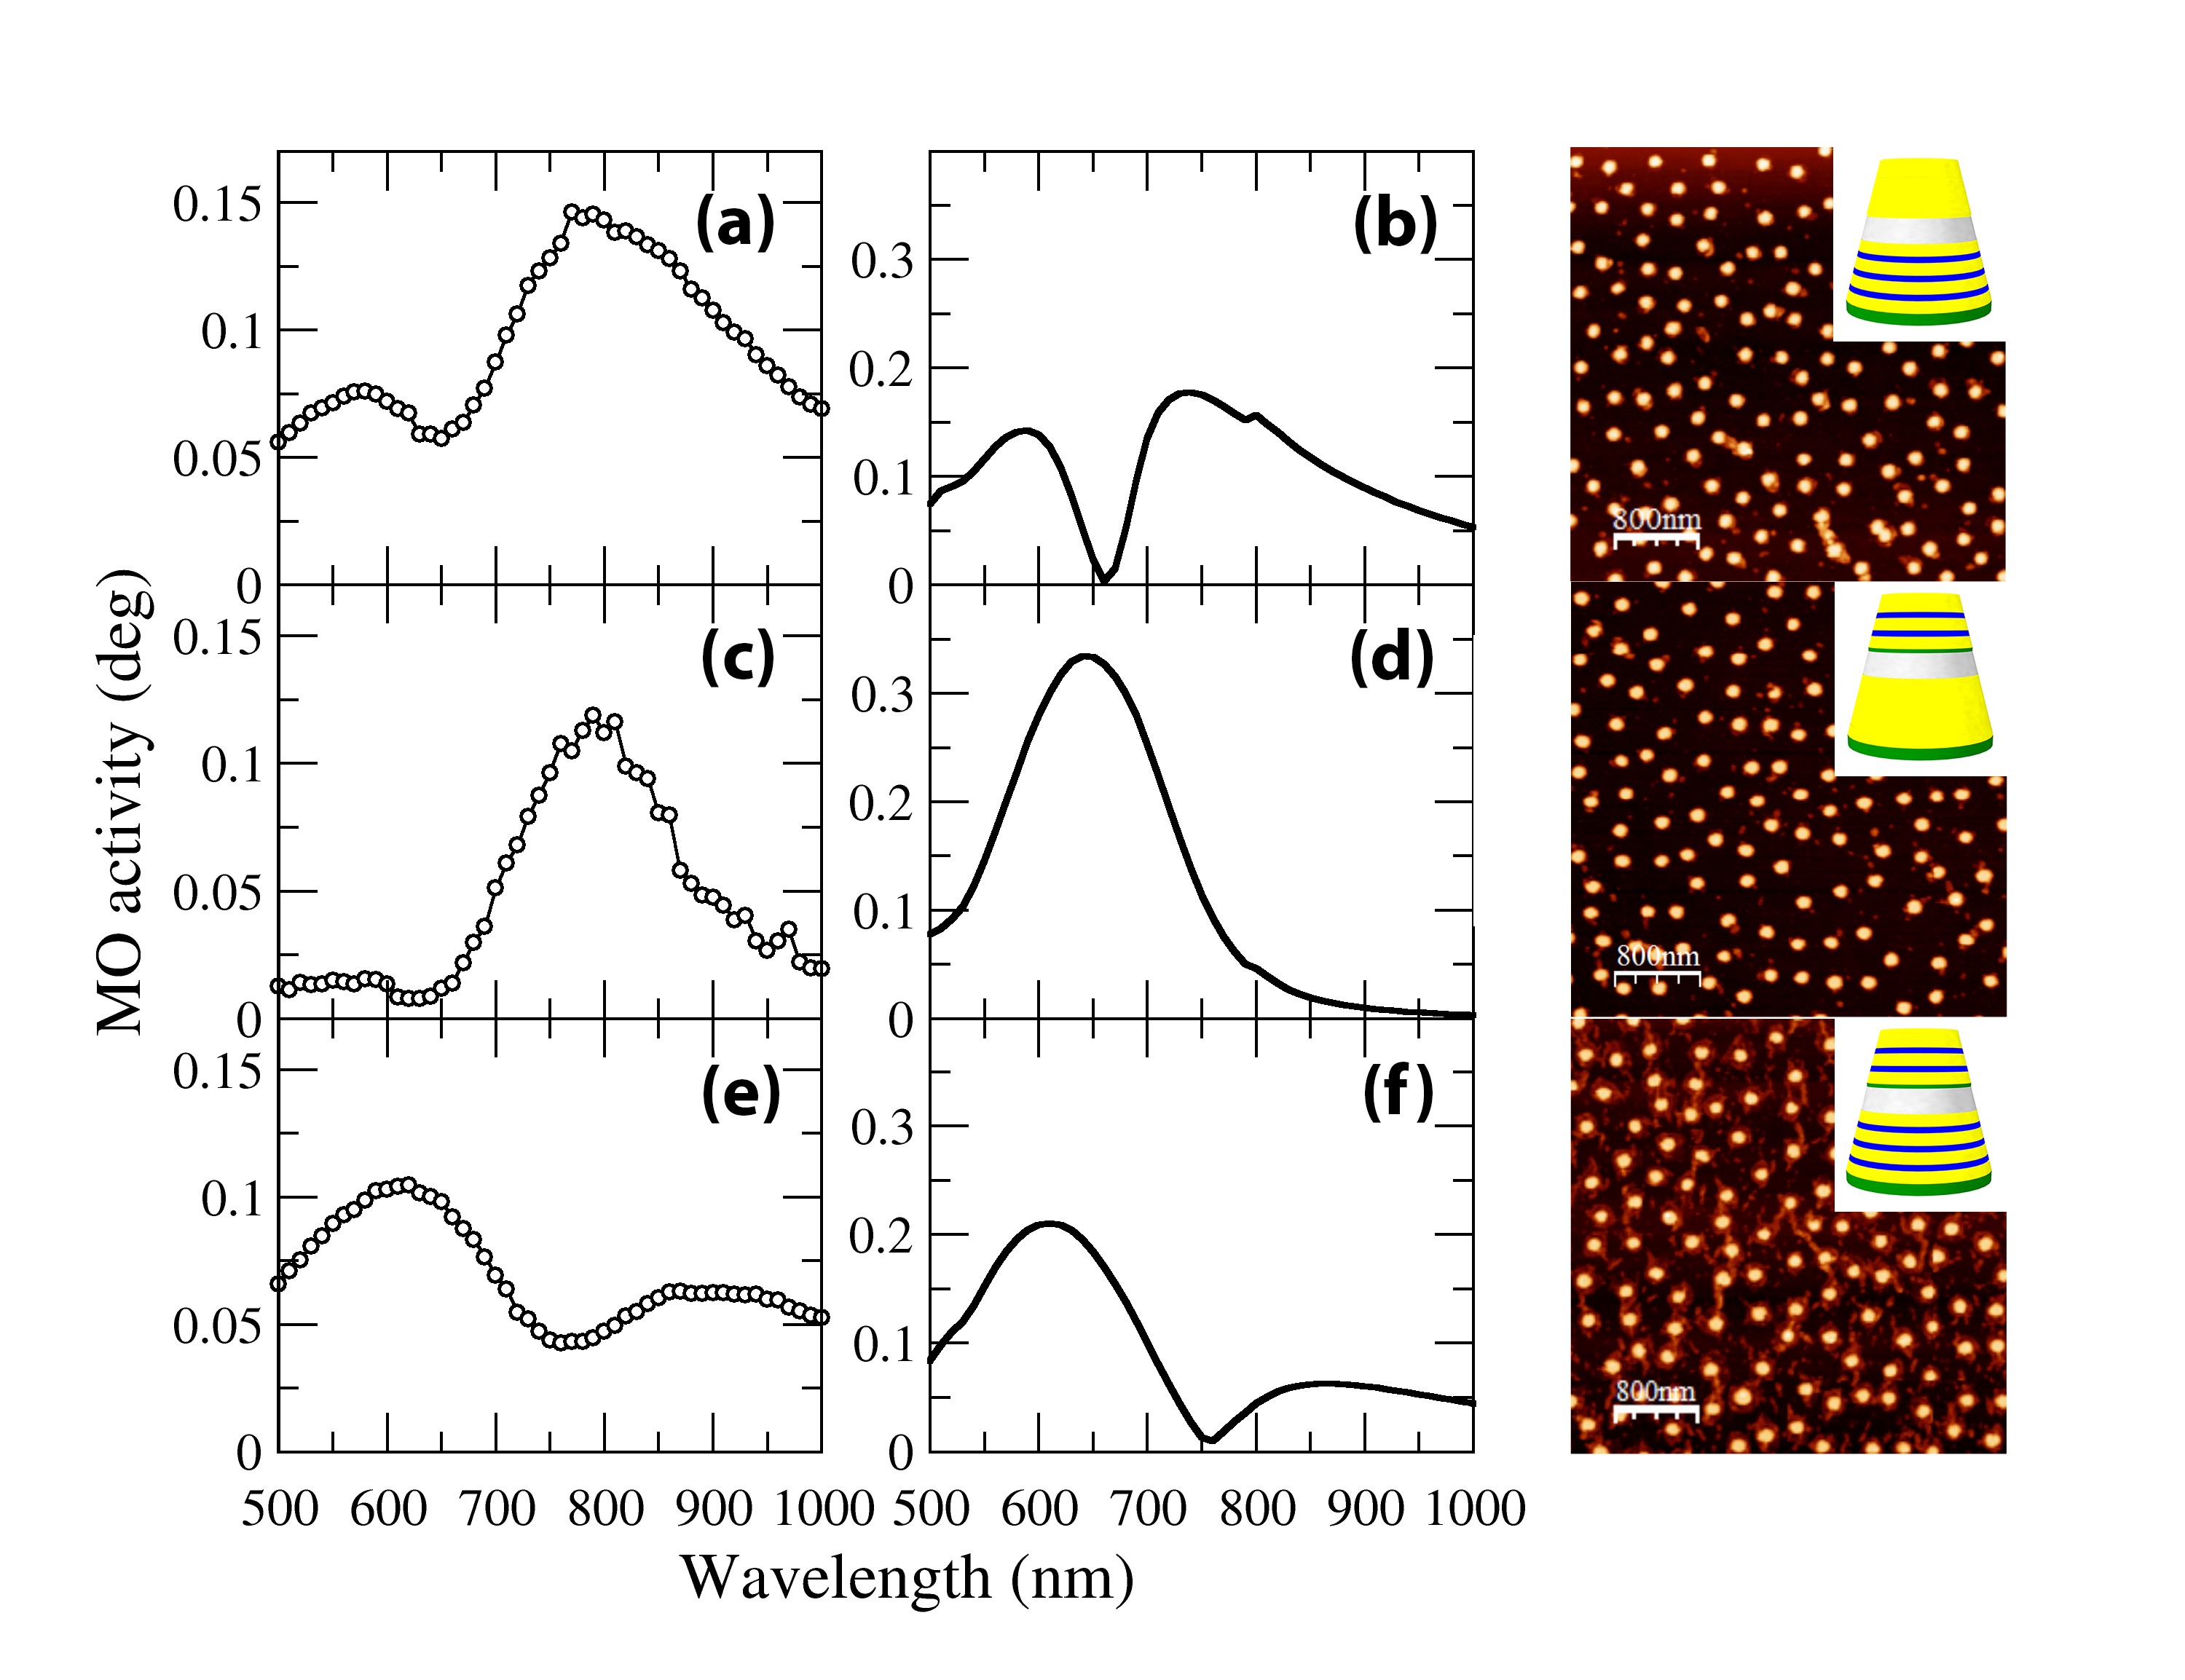
\includegraphics[width=1\columnwidth]{chapter_4/graphics/F4_MOA_3x3_finalR1.png}
\caption{Experimental results (a) and numerical simulations (b) of the MO activity when the MP disk is at the bottom, (c),(d) are the same but when the MP disk is at the top, and (e),(f) when both are MP. In the rightmost panel we show Atomic Force Microscopy (AFM) images of the three experimental samples where the density of disks (about $15\%$ coverage) and homogeneity can be seen. The images show that the disk diameter ranges from $130nm$ to $150nm$. Also is represented a scheme of the structures. In green we depict the $\textnormal{Ti}$ adhesive layer, in blue the $\textnormal{Co}$ layers, grey is the $\textnormal{SiO}_{2}$ and yellow are the gold layers. The three different systems are constituted by two metallic disks separated by $20nm$ of $\textnormal{SiO}_{2}$. For the configuration with the MP disk at the bottom (top panels), the MP disk is composed of a $2nm$ $\textnormal{Ti}$ layer followed by a $4nm$ $\textnormal{Au}$ layer and three sequential combinations of $2nm$ $\textnormal{Co}/4nm$ $\textnormal{Au}$ layers. The disk at the top is composed by $16nm$ $\textnormal{Au}$. For the configuration with MP disk at the top, the MP disk is composed by an initial $1nm$ layer of $\textnormal{Ti}$ then $4nm$ $\textnormal{Au}$ layer and two sequences of $2nm$ $\textnormal{Co}/4nm$ $\textnormal{Au}$ layers. The disk at the bottom is composed by $22nm$ of $\textnormal{Au}$. When both disks are MP, they consist of those $\textnormal{Au}/\textnormal{Co}$ sequences employed in the other two situations. \label{chap5:Experim}}
\end{figure}

Despite the simplicity of the two interacting dipoles model, it describes quite well the outcome of the interaction between disks in magnetoplasmonic dimers. For example, in Fig. (\ref{chap5:Experim}), we present the experimental MO activity for three different samples. They consist of a layer of two metallic disks separated by $\approx 20 nm$ of $\textnormal{SiO}_2$.  deposited on a glass substrate. The three samples have a homogeneous distribution of the disks, with a filling factor of $15\%$. The diameter of the disks ranges from $130$ to $150nm$. They were obtained by hole mask colloidal lithography, metal evaporation, and lift off \cite{fredriksson2007hole}. The internal structure of the disks is presented in the rightmost panel of Fig.  (\ref{chap5:Experim}), with the disk's dimensions in the caption. In the upper panel, the bottom disk consists of a $\textnormal{Au}/\textnormal{Co}$ multilayer (MP) and the top one is a $\textnormal{Au}$ disk (P); in the middle panel, the top disk is a $\textnormal{Au}/\textnormal{Co}$ multilayer (MP) and the bottom one is a $\textnormal{Au}$ disk (P); and, finally, in the lower panel, both disks are $\textnormal{Au}/\textnormal{Co}$ multilayers (MP).\\
As can be observed, when the bottom disks are magnetoplasmonic, \textit{i.e.}, upper and lower panels on the righthand side of Fig. (\ref{chap5:Experim}), the MOA spectrum has two peaks. Despite the lower $\textnormal{Co}$ content of the upper panel, the lower-energy peak has a higher intensity in this sample than in the lower panel, where the two disks are magnetoplasmonic. Moreover, the MOA spectrum of the middle panel has only one peak, whose intensity is also greater than the intensity of the low-energy peak of the lower panel. Additionally, in Fig. (\ref{chap5:Experim}), we also present a FDTD theoretical calculation which takes into account the internal structure of the disks. As can be observed, these calculations reproduce quite well the experimental behaviour, and the results are also equivalent to those obtained with the previously exposed analytical approach for intermediate interactions presented in Fig. (\ref{HighInt}). The numerical calculations have been made using $130nm$ for the diameter of the base of the cone and $100nm$ for the top in all cases. An increase in these numbers would cause a redshift of the peaks.

\section{Conclusion}

In conclusion, we have analysed the effect of electromagnetic interactions on the MO response of magnetoplasmonic dimers composed of two metallic disks separated by a dielectric. The MO response strongly depends on the plasmonic versus magnetoplasmonic nature of the two disks, observing for specific configurations that the MO response can be dominated by the induced MOA of the purely plasmonic disk. On the other hand, the MO activity of a system with only one of the disks containing material with intrinsic MO can be even larger than that of a system composed of two MP disks. A simple analytical model of two interacting point dipoles allows us to fully describe separately the contribution of each disk to the optical and MOA of the system, along with the relative phases of the dipoles responsible for these activities. Experimental results and numerical calculations fully support the analytical calculations results.


%\bibliographystyle{plain}
%\bibliography{References}